%%%%%%%%%%%%%%%%%%%%%%%%%%%%%%%%
% Chap 2. Preliminaries
%%%%%%%%%%%%%%%%%%%%%%%%%%%%%%%%

\chapter{Preliminaries} \label{chapter2}

This chapter presents the necessary background and mathematical tools required for the subsequent chapters.
Since the proposed controller (constrained optimization-based neuro-adaptive controller (CoNAC)) is based on adaptive control and constrained optimization theory and deep neural networks (DNNs), this chapter covers the following topics: control theory, constrained optimization theory, and the approximation theory.

%%%%%%%%%%%%%%%%%%%%%%%%%%%%%%%%
\section{Related Control Theory} \label{chap2:sec:ctrl}
%%%%%%%%%%%%%%%%%%%%%%%%%%%%%%%%

% \subsection{Backstepping Control} \label{chap2:sec:BSC}

In this thesis, the Euler-Lagrange systems will be used as target system since many engineering systems can be modeled using Euler-Lagrange systems (\eg aerospace, robotics, and automotive applications).
Using system matrices $M(q)\in\R^{n\times n}$, $C(q,\dot{q})\in\R^{n\times n}$, and $G(q)\in\R^{n}$, and external forces $F(q)\in\R^n$, the Euler-Lagrange system can be rewritten as
\begin{equation}
    M(q)\ddot{q} + C(q,\dot{q})\dot{q} + G(q) +F(q)= \tau
    \label{chap2:eq:EL}
\end{equation}
where $q\in\R^n$ denotes generalized state variables and $\tau\in\R^n$ denotes generalized control input.
The Euler-Lagrange system can be transformed into a second-order control-affine system by defining the state variables $x_1\triangleq q$ and $x_2\triangleq \dot q$ as
\begin{equation}
  \begin{aligned}
    \dot x_1 =& x_2\\
    \dot x_2 =& f(x,t)+g(x,t)u
  \end{aligned}
\end{equation}
where $x\triangleq [x_1,x_2]^T\in\R^{2n}$, $u\triangleq \tau$, $f(x,t)\triangleq M^{-1}(-Cx_2-G-F)$ and $g(x,t)\triangleq M^{-1}$ are system functions.

Using backstepping control approach, the system can be broken down into lower dimension subsystem by generating the auxiliary control input to regulate the higher dimension original system \cite{RN7}.
Considering tracking error with a given smooth reference signal $r_1(t)\in\R^n$, the tracking error and its time-derivative are defined as
\begin{equation}
  e_1\triangleq x_1-r_1,\quad \dot e_1= \dot x_1-\dot r_1=x_2-\dot r_1
  .
\end{equation}
Using the Lyapunov function defined as $\mathcal V_1\triangleq (1/2)e_1^Te_1$, the time-derivative of $\mathcal V_1$ yields
\begin{equation}
  \dot {\mathcal V}_1 =e_1^T\dot e_1=e_1^T(x_2-\dot r_1)
\end{equation}
The auxiliary control input $r_2\in\R^n$ which realizes $\dot{\mathcal V}_1<0$ can be defined as $r_2\triangleq  -k_1e_1+\dot r_1$ for some constant $k_1\in\R_{>0}$.
Let $e_2\triangleq x_2-r_2=x_2-(-k_1e_1+\dot r_1)$ denotes the tracking error of $x_2$.

Then, the time-derivative of the Lyapunov function $\mathcal V_2\triangleq (1/2)e_1^Te_1+(1/2)e_2^Te_2$ yields
\begin{equation}
  \begin{aligned}
    \dot {\mathcal V}_2
    =&
    e_1^T(x_2-\dot r_1)+e_2^T\dot e_2\\
    =&
    e_1^T(-k_1e_1+e_2)+e_2^T\dot e_2\\
    =&
    -k_1e_1^Te_1+e_1^Te_2+e_2^T(f+gu-\dot r_2)\\
    .
  \end{aligned}
\end{equation}

Therefore, the stabilizing control input $u$ that realizes $\dot {\mathcal V}_2=-k_1e_1^Te_1-k_2e_2^Te_2<0$ can be designed as
\begin{equation}
  u\triangleq g^{-1} (-e_1 -k_2e_2 +\dot r_2 -f)
\end{equation}
where $k_2\in\R_{>0}$ is a positive constant.
Note that, the stabilizing control input $u$ requires the knowledge of the system functions $f(x)$ and $g(x)$.

On the other hand, the bounded input bounded output (BIBO) stability defined in Theorem \ref{chap2:thm:BIBO}, will be used for the stability analysis in the later chapters.

\begin{theorem}(see \cite[Theorem 1.9]{RN23})
  Let the closed-loop transfer function $H(x)$ be the exponentially stable and strictly proper.
  Then $y = H\star u\in L^\infty$, $\dot y\in L^\infty$, and $y$ is uniformly continuous, if $u\in L^\infty$.
  \label{chap2:thm:BIBO}
\end{theorem}

In other word, $\Vert x\Vert$ is bounded, for a linear system $\dot x=Ax+Bu$ where $A$ is Hurwitz matrix and $\Vert B\Vert_F$ and $\Vert u\Vert$ are bounded.
Without loss of generality, the BIBO stability can be extended to matrix state $x\in\R^{n\times m}$ as well.

%%%%%%%%%%%%%%%%%%%%%%%%%%%%%%%%
\section{Mathematical Review} 
%%%%%%%%%%%%%%%%%%%%%%%%%%%%%%%%

\subsection{Matrix Algebra} 

In this thesis, we will use the following notations for matrix algebra.
\begin{itemize}
  \item $x_{(i)}$ denotes the $i$-th element of vector $x\in\mathbb R^n$.
  \item $A_{(i,j)}$ denotes the element in the $i$-th row and $j$-th column of matrix $A\in\R^{n\times m}$.
  \item $\text{row}_j(A)$ denotes the $j$-th row of matrix $A\in\R^{n\times m}$.
  \item $\lambda_\text{min}(A)$ denotes the minimum eigenvalue of matrix $A\in\R^{n\times n}$.
\end{itemize}

For a matrix $A\in\mathbb R^{n\times m}$, the \textbf{vec} operator is defined as
\begin{equation}
  \text{vec}(A) \triangleq 
  \begin{bmatrix}
      \text{row}_1(A^T) & \text{row}_2(A^T) & \cdots & \text{row}_n(A^T)
  \end{bmatrix}
  \in\mathbb R^{nm}
  .
\end{equation}

Moreover, for the brief expression of neural networks (NNs) and their gradient, \textbf{Kronecker product} will be used which is defined in Definition \ref{chap2:prop:kron}.

\begin{definition}[see {\cite[Definition 7.1.2]{RN22}}]
  Using the \textbf{vec} operator, the \textbf{Kronecker product} of two matrices $A\in\mathbb R^{n\times m}$ and $B\in\mathbb R^{p\times q}$ is defined as
  \begin{equation}
      A\otimes B\triangleq 
      \begin{bmatrix}
        A_{(1,1)}B & A_{(1,2)}B & \cdots & A_{(1,m)}B \\
        A_{(2,1)}B & A_{(2,2)}B & \cdots & A_{(2,m)}B \\
        \vdots & \vdots & \ddots & \vdots \\
        A_{(n,1)}B & A_{(n,2)}B & \cdots & A_{(n,m)}B
      \end{bmatrix}
      \in\mathbb R^{np\times mq}
      .
  \end{equation}
\end{definition}

The \textbf{Kronecker product} has the following proposition.

\begin{proposition}[see {\cite[Proposition 7.1.9]{RN22}}]
  For matrix $A\in\mathbb R^{n\times m}$ and vector $x\in\mathbb R^n$, we have the following property
  \begin{equation}
    A^Tx = \text{vec}(A^Tx) = \text{vec}(x^TA) = (I_m\otimes x^T)\text{vec}(A)
    .
  \end{equation}
  \label{chap2:prop:kron}
\end{proposition}
The proof of Proposition \ref{chap2:prop:kron} can be found in \cite{RN22}.
Using Proposition \ref{chap2:prop:kron} the gradient with respect the vectorized $A$ can be computed as
\begin{equation}
  {\partial (A^Tx)\over\partial \text{vec}(A)} = I_m\otimes x^T
  .
\end{equation}

The reader is referred to \cite[Chapter 7]{RN22} for more details about the \textbf{Kronecker Product} and its properties.

\subsection{Constrained Optimization Theory} 

The general formulation of the constrained optimization problem can be represented as 
\begin{equation}
    \underset{x}{\text{minimize}}\quad f(x),
    \quad\quad
    \text{subject to}
    \begin{cases}
      c_j(x)= 0,    & \forall j\in\mathcal E\\
      c_j(x)\leq 0, & \forall j\in\mathcal I 
    \end{cases}
\end{equation}
where $f:\mathbb R^n\to\mathbb R$ denotes the objective function, $x\in\mathbb R^n$ denotes the optimization variables, and $\mathcal E$ and $\mathcal I$ are the set of equality and inequality constraints, respectively.
The objective of the constrained optimization problem is to find the optimal point $x^*$ that locally or globally minimizes the objective function $f(x)$, satisfying the constraints $c_j(x)$.
Generally, the imposed constraints in an active set $\mathcal A\triangleq\mathcal E \cup \{j\in\mathcal I\ \vert \ c_j\ge0\}$ are supposed to satisfy the Linear Independence Constraint Qualification (LICQ) which is defined in Definition \ref{chap2:def:LICQ}.

\begin{definition}[see {\cite[Definition 12.1]{RN9}}]
  If the gradients of the active constraints $\nabla c_j(x^*)$, $j\in\mathcal A$, are linearly independent, the set of constraints $\{c_j\}$ satisfies the \textit{Linear Independence Constraint Qualification} (LICQ) at $x^*$.
  \label{chap2:def:LICQ}  
\end{definition}

Using the Lagrange multipliers $\lambda_j$ for each constraint $c_j(x)$, the Lagrangian function is defined as
\begin{equation}
    L(x,[\lambda_j]_{j\in\mathcal E\cup\mathcal I}) = f(x) + \sum_{j\in\mathcal E}\lambda_jc_j(x) + \sum_{j\in\mathcal I}\lambda_jc_j(x)
    .
\end{equation}
Then, the constrained optimization problem can be reformulated as the min-max problem as
\begin{equation}
  \min_x \max_{[\lambda_j]_{j\in\mathcal E\cup\mathcal I}} L(x, [\lambda_j]_{j\in\mathcal E\cup\mathcal I})
  .
\end{equation}

The conditions of optimality are defined by the first-order necessary condition and the second-order necessary and sufficient conditions.
The first-order necessary condition which is often known as the \textit{Karush-Kuhn-Tucker conditions} (KKT) is that the gradient of the Lagrangian function $L$ at $(x^*,\lambda^*)$ should be zero.
The second-order necessary condition is that the Hessian matrix of $L$ at $(x^*,\lambda^*)$ should be positive semi-definite while the second-order sufficient condition is that the Hessian matrix should be positive definite (\ie $L$ is convex in the neighbor of the point $(x^*,\lambda^*)$).
The constrained optimization problem typically attempts to find local solution ($x^*,\lambda^*$) which satisfy the first-order necessary condition of optimality, since there is no guarantee that $L$ is convex function (\ie for the global optimality second-order condition is required).
The KKT conditions for the constrained optimization problem is stated in \cite{RN9} as following Theorem \ref{chap2:thm:KKT}.

\begin{theorem}[see {\cite[Theorem 12.1]{RN9}}]
  Let $x^*$ be a local solution of the constrained optimization problem. 
  Then, there exists a Lagrange multiplier vector $\lambda^*$ such that the following conditions are satisfied:
  % \begin{subequations} 
  \begin{equation}
    \begin{aligned}
      \nabla_x L(x^*,\lambda^*) &= 0\\
      c_j(x^*) &= 0, \quad \forall j\in\mathcal E\\
      c_j(x^*) &\leq 0, \quad \forall j\in\mathcal I\\
      \lambda_j^* &\geq 0, \quad \forall j\in\mathcal I\\
      \lambda_j^*c_j(x^*) &= 0, \quad \forall j\in\mathcal E\cup\mathcal I
      .
    \end{aligned}
  \end{equation}
  % \end{subequations}
  \label{chap2:thm:KKT}
\end{theorem}
For the details of the optimization theory, the reader can refer to \cite{RN9} and \cite{RN1}.

\subsection{Preservation of Convexity} \label{chap2:sec:convex_preserve}

\begin{definition}[see {\cite[Chapter 2.1.4]{RN1}}]
  A set $C$ is \textbf{convex} if the line segment between any two points in $C$ lies entirely in $C$. That is, for all $x$, $y\in C$ and $\lambda\in [0,1]$, we have
  \begin{equation}
      \lambda x + (1-\lambda)y \in C
      .
  \end{equation}
\end{definition}

\begin{definition}[see {\cite[Chapter 3.1.1]{RN1}}]
  A function $f:\mathbb R^n\to \mathbb R$ is \textbf{convex} if \textbf{dom} of $f$ is a convex set and if for all $x$, $y\in \textbf{dom}\ f$ and $\lambda\in [0,1]$, we have
  \begin{equation}
      f(\lambda x + (1-\lambda)y) \leq \lambda f(x) + (1-\lambda)f(y)
      .
  \end{equation}
\end{definition}

The convexity is very useful property in optimization theory and controller design to find optimal control parameters, since the every local solution points are global solution point satisfying the second-order necessary and sufficient conditions \cite[Theorem 2.5]{RN9}.
Furthermore, if the optimal point of the convex function $f(x)$ is the origin, the opposite direction of the gradient of $f$ at $x$ is the descent direction.
In other word, the angle between the gradient at $x$ and the vector $x$ is positive as following Lemma \ref{chap2:lem:conv_ang}.

\begin{lemma}
  Let $f:\mathbb R^n\to \mathbb R$ be a convex function and $x$ be a point in the domain of $f$.
  If the origin is the optimal point of the function $f$, then the angle between the gradient of $f$ at $x$ and the vector $x$ is positive, implying that $\nabla f^Tx>0$.
  \label{chap2:lem:conv_ang}
\end{lemma}

\begin{proof}
  Let the origin be the isolated optimal point that minimizes the function $f$ such that $f(x) > f(0)$.
  Then, the following inequality holds:
  \begin{equation}
      \begin{aligned}
          \nabla f^T (-x)
          =&
          {d\over d\delta } f( x -\delta x)\bigg\vert _{\delta=0} \\
          =& \lim_{\delta\to 0} {f( x+\delta (0-x) - f( x)\over \delta}\\
          \le& \lim_{\delta\to0} {\delta f(0) + (1-\delta) f( x )-f( x)\over \delta}
          \\
          =& f(0) - f( x) < 0
          \end{aligned}
          .
  \end{equation}
  It implies that the angle between the gradient of $f$ at $x$ and the vector $x$ is positive.
\end{proof}

In \cite[Chapter 2.3.2]{RN1}, the authors stated that the affine functions preserve the convexity of the function as follows:
\begin{displayquote}
  
  Recall that a function $f:\R^n\to\R^m$ is affine if it is a sum of a linear function and a constant, \ie if it has the form $f(x) = Ax + b$, where $A\in\R^{m\times n}$ and $b\in\R^m$. Suppose $S\in\R^n$ is convex and $f:R\in n\to\R^m$ is an affine function. Then the image of $S$ under $f$,
  \begin{equation}
    f(S) = \{ f(x) | x\in S \}
    ,
  \end{equation}
  is convex.

\end{displayquote}
This property will be utilized in the stability analysis of the controller in Chapter \ref{chapter4}.

%%%%%%%%%%%%%%%%%%%%%%%%%%%%%%%%
\section{Deep Neural Networks}
%%%%%%%%%%%%%%%%%%%%%%%%%%%%%%%%

% \subsection{Universal Approximation Property} 

The capability of NNs to approximate functions is based on the approximation theory \cite{RN4}. 
In other words, the NNs can approximate any sufficiently smooth function on a compact set with arbitrary accuracy according to the universal approximation theorem defined in Theorem \ref{chap2:thm:uni_approx}.

\begin{theorem}[see {\cite{RN48, RN43}}]

  Let $f$ be a sufficiently smooth function defined on a compact set $x\in\Omega\in\R^n$.
  Then, for any $\epsilon\in\R_{>0}$, there exists an ideal weight vector $\theta^*$ in a single hidden layer NN (SHLNN) with the sigmodal activation function $\Phi(x;\theta^*)$ that approximates $f$ with $\epsilon$-accuracy in $x\in\Omega$ such that $\sup_{x\in\Omega}\Vert \Phi(x;\theta^*) - f(\cdot) \Vert = \epsilon < \infty$.

  \label{chap2:thm:uni_approx}
\end{theorem}

Besides, the universal approximation property of deep NNs (DNNs) is also reported in \cite{RN70}.
Generally, the ideal vector is assumed to be constant and bounded such that $\Vert\theta^*\Vert\le \bar\theta <\infty$.

\subsubsection{Mathematical Expression of Deep Neural Network} \label{chap2:sec:DNN}

Most literature which utilizes the SHLNNs in the controller, have shown that the SHLNNs can approximate the uncertain system functions or control law with satisfactory performance index.
However, the DNNs are exponentially more expressive than the SHLNNs to the same accuracy in terms of the total number of weights \cite{RN65}.
Therefore, the DNNs will be utilized in the controller in this thesis.
Note that the SHLNN can be considered as the simplest architecture of the DNN with a single hidden layer.

\begin{figure}[!t]      
  \centering
  % {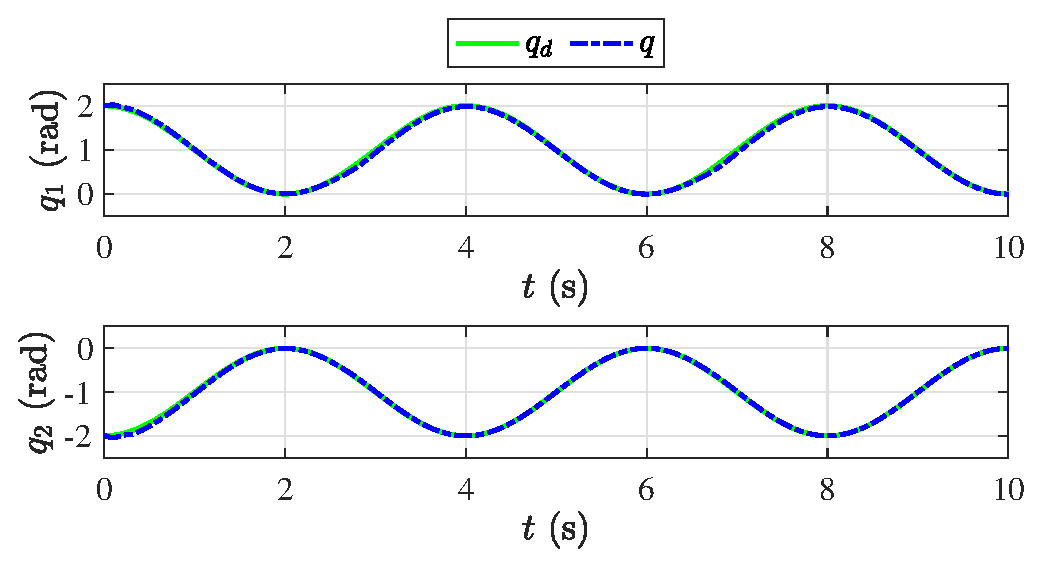
\includegraphics[width=.85\linewidth]{fig4.eps}}
  {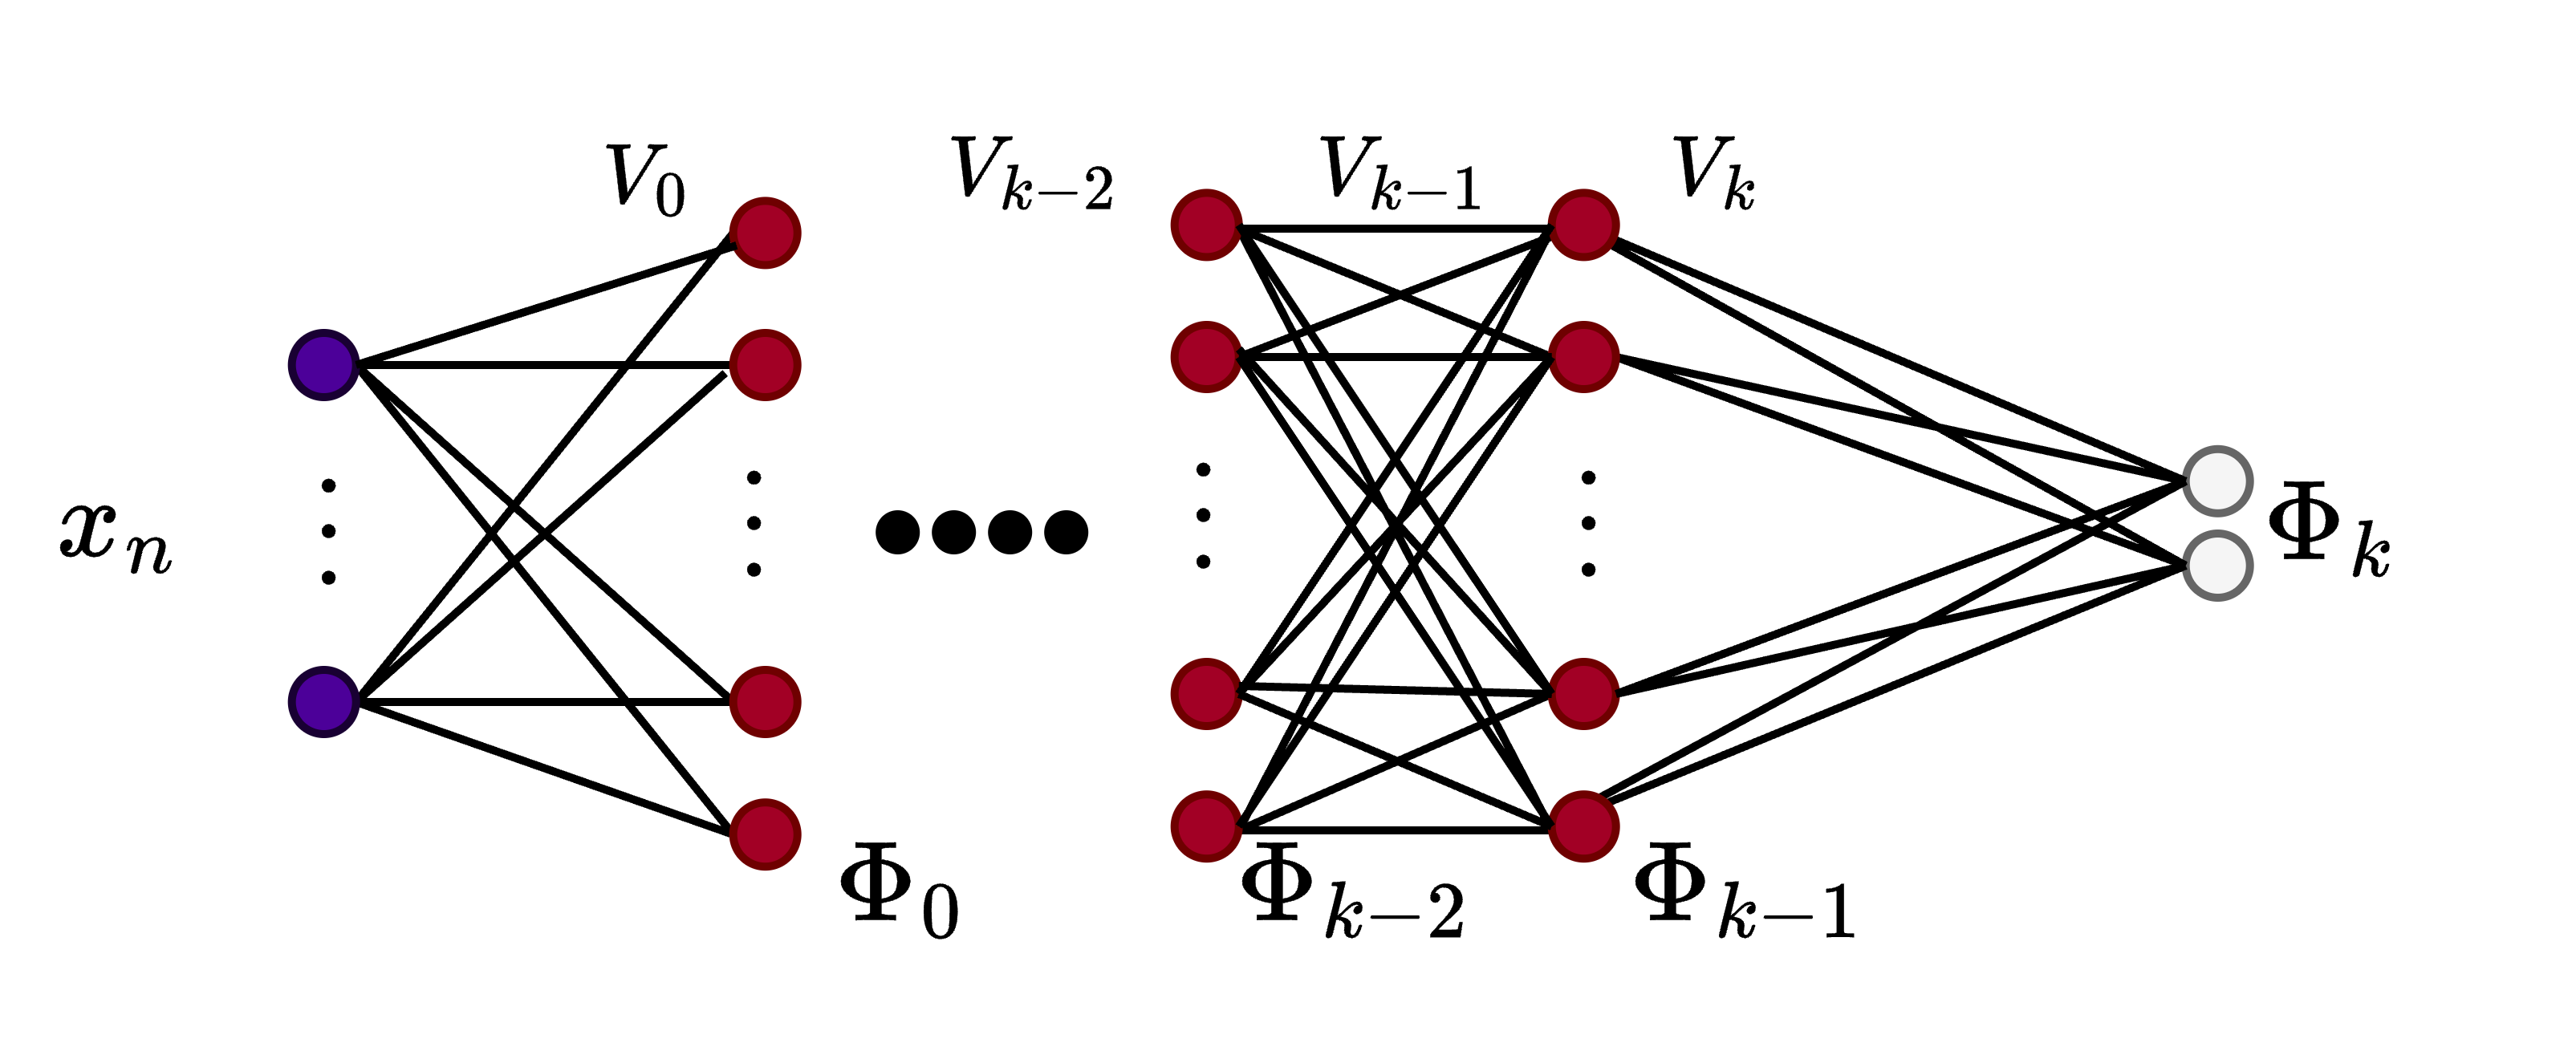
\includegraphics[width=.85\linewidth]{imgs/NN.drawio.png}}
  \caption{Architecture of the deep neural network (DNN).}
  \label{chap2:fig:DNN}
\end{figure}

In general, it was open problem to leverage the DNNs in controllers due to the nonlinearity and mathematically complex architecture of the DNNs.
In \cite{RN13}, Omkar Sudhir Patil \etal proposed the novel DNN based neuro-adaptive control for control-affine nonlinear systems.
The architecture of the DNN in the controller is described in Fig.~\ref{chap2:fig:DNN} and is defined as 
\begin{equation}
  \Phi(x_n;\theta) \triangleq 
  \underbrace{
    V_k^T  \phi_{k}(
    \underbrace{
      V_{k-1}^T   \cdots \phi_2(
      \underbrace
        {
        V_1^T   \phi_1(
        \underbrace
          {
          V_0^T   x_n
        }_{\Phi_0}
        )
      }_{\Phi_1}
      )\cdots )
    }_{\Phi_{k-1}}
    )
  }_{\Phi_k}
  \label{chap2:eq:DNN}
\end{equation}
where $x_n$ denotes the NN input vector, $V_i\in\R^{(l_i+1)\times l_{i+1}}$ is the weight matrix of the $i\textsuperscript{th}$ layer, and $\phi_i: \R^{l_i}\to\R^{l_i+1}$ represents the activation function of the $i\textsuperscript{th}$ layer. 
The element-wise activation function is defined as $\phi_i(x)=[\sigma(x_{(1)}),\sigma(x_{(2)}),\cdots, \sigma(x_{(l_{i})}), 1]^T$, where $\sigma: \R\to\R$ is a nonlinear function, and the augmentation of $1$ is used to account for bias terms in the weight matrices.  
For a better understanding, \eqref{chap2:eq:DNN} also can be represented recursively as 
\begin{equation}
    \Phi_i \triangleq
    \begin{cases}
        V_i^T  \phi_i(\Phi_{i-1}), &i\in[1,\dots,k],\\
        V_0^T  x_n,&i=0,
    \end{cases}
\end{equation}
where $\Phi_i$ denote each layer's output (\ie the last layer's output is equal to the output of DNN such that $\Phi_k = \Phi(x_n;\theta)$).

One of the widely used activation functions for large DNNs is from the ReLU family \cite{RN15}, which effectively avoids the gradient vanishing problem during error backpropagation. 
The gradient vanishing problem occurs when the gradient of the activation function is close to zero, since the gradient of each layer is multiplied using chain rule to backpropagate the error to the inner layers (\ie deeper NNs have high possibility of gradient vanishing).
However, for control applications where relatively shallow DNNs are typically sufficient, and the gradient vanishing issue is less severe, the sigmoid function or the hyperbolic tangent function is commonly used as the activation function. 
These functions simplify stability analysis due to their continuous differentiability, and their outputs and gradients are bounded such that $\Vert \phi_i(\cdot)\Vert < \infty$ and $\Vert \nabla\phi_i(\cdot)\Vert_F < \infty$. 
In this thesis, the hyperbolic tangent function $\tanh(\cdot)$ was selected as the activation function (\ie $\sigma(\cdot) = \tanh(\cdot))$, which provides desirable boundedness with $\Vert\sigma(\cdot)\Vert<1$ and $\Vert\nabla\sigma(\cdot)\Vert< 1$.
Note that, the number of hidden layers should be limited around 5 to avoid the gradient vanishing issue, since the gradient vanishing problem is not addressed.

For simplicity, each layer's weights are vectorized as $\theta_i\triangleq\text{vec}(V_i)\in\R^{\Xi_i}$, where $\Xi_i\triangleq (l_i+1)l_{i+1}$ is the number of weights in the $i\textsuperscript{th}$ layer. 
The total weight vector $\theta\in\R^{\Xi}$ is defined by augmentation $\theta_i$ for all $i\in \left[0,\cdots,k\right]$ as 
\begin{equation}
    \theta \triangleq 
    \begin{bmatrix}
        \theta_k\\
        \theta_{k-1}\\
        \vdots\\
        \theta_0
    \end{bmatrix}
    =
    \begin{bmatrix}
        \text{vec}(V_k)\\
        \text{vec}(V_{k-1})\\
        \vdots\\
        \text{vec}(V_0)
    \end{bmatrix},
\end{equation}
where $\Xi={\sum_{i=0}^{k} \Xi_i}$ represents the total number of weights. 

\subsubsection{Gradient of Deep Neural Network} \label{chap2:sec:DNNgrad}

In the derivation of adaptation law, the gradient of the DNN with respect to the weights is required.
The gradient of $ \Phi(x_n;\theta)$ with respect to $\theta$ is defined as
\begin{equation}
    {\partial\Phi\over\partial \theta}=
    \begin{bmatrix}
        \dfrac{\partial \Phi}{\partial \theta_k}&
        \dfrac{\partial \Phi}{\partial \theta_{k-1}}&
    \cdots &
        \dfrac{\partial \Phi}{\partial \theta_0}
    \end{bmatrix}
    \in\R^{n \times \Xi}
    \label{chap2:eq:DNNgrad}
\end{equation}
where
\begin{equation}
    \frac{\partial \Phi}{\partial \theta_i} = 
    \begin{cases}
        (I_{l_{k+1}}\otimes \phi_{k}^T  ), & i=k \\
        V_k^T   \phi_{k}' (I_{l_{k}}\otimes  \phi_{k-1}^T  ), & i=k-1\\
        &\vdots \\
        V_k^T   \phi'_{k} \cdots V_1^T  \phi_1' (I_{l_1}\otimes x_n^T  ), & i = 0
    \end{cases},
\end{equation}
where $\phi_i\triangleq \phi_i(\Phi_{i-1})$ and $\phi_i'\triangleq \partial \phi_i/\partial \Phi_{i-1}$.
The gradient can be obtained using the chain rule and Proposition \ref{chap2:prop:kron}.
